\chapter{Bibliographic Research} \label{lab:ch3-bibliographic-research}

This chapter will go through the main ideas, principles, algorithms, and notions used throughout the implementation of \app{}.
They will be presented as found in literature, with references to bibliographic sources, hence the chapter's title.
While the sections don't necessarily come in a given order, I tried to structure them from the main ideas to the more detailed aspects.
Each section can be read in isolation, so feel free to jump to the one of your interest.



\section{Existing Solutions}

In this section I will present software solutions (sometimes backed by hardware) which solve a similar problem to what \app{} aims to solve.
They will be presented in comparison with \app{}, so you will see both arguments for and against my solution.
Frankly, I found no other project doing exactly what I do, so none of the presented solutions will be a one-to-one match to my project.
Also, when comparing, keep in mind that \app{} is developed by a single person, in a limited amount of time, and serves more as a proof of concept rather than a polished end product.

Without further ado, lets dive deep into the ``opponents'' of \app{}.



\subsection{YubiKey} \label{lab:c3-yubikey}
The YubiKey is a product if the company called yubico.
It has gained rising popularity over the last few years, both for personal and professional use.
It comes in various shapes and forms, but mostly resembles a USB stick.
However, these are custom-built hardware designed specifically to support different protocols which need a security key.

Citing from their website \cite{yubikey},
``The YubiKey works with hundreds of enterprise, developer and consumer applications, out-of-the-box and with no client software.
Combined with leading password managers, social login and enterprise single sign on systems the YubiKey enables secure access to thousands of online services.''
Their products also support OTP:
``OTP supports protocols where a single use code is entered to provide authentication.
These protocols tend to be older and more widely supported in legacy applications.
The YubiKey communicates via the HID keyboard interface, sending output as a series of keystrokes.
This means OTP protocols can work across all OSs and environments that support USB keyboards, as well as with any app that can accept keyboard input.''

Their most recommended product is YubiKey 5, and they call it the world's number one multiprotocol security key.
From these series, as of August 21st, 2026, the cheapest for 70.18 EUR.
Other models from this series go even more expensive, with the biggest price being 102.85 EUR.
The models differ in capabilities, but also physical size, the smaller ones costing generally more.

Yubico is a generally trusted company with a good reputation.
It is based in Stockholm, Sweden, and was founded in 2007 by Stina Ehrensvard.
According to Tracxn\footnote{\url{https://tracxn.com/d/companies/yubico/__fgcOVhxhBthY3y9De52Otl021ENbj9VtVBf2Ho1uoOI\#about-the-company}}, it is ranked 1st among its competitors.
They have around 300 employees and have a total of 30M USD funding.
However, the software that runs in YubiKey is closed-source.
They did have some security issues in the past\footnote{\url{{https://en.wikipedia.org/wiki/YubiKey\#Security_issues}}}, including:
\begin{itemize}
    \item \b{ROCA vulnerability - October 2017}.
        A vulnerability which affected many security keys which implemented RSA.
        It allowed an attacker to reconstruct the private key by using the public key.
        Yubico gave free replacements with newer series devices.
    \item \b{OTP password protection - January 2018}
        This affected a specific model, the YubiKey NEO.
        The password protection for the OTP functionality could be bypassed.
        Yubico offered a firmware update and free replacements.
    \item \b{Cloning vulnerability - September 2024}
        It allowed a person to clone a YubiKey if they gave physical access.
        It was remediated through a firmware update.
        This required advanced cryptographic and technical knowledge: they looked at the electromagnetic emissions of the keys. \cite{eukleak}
\end{itemize}

In comparison with \app{}, YubiKeys are much more secure, since they are specialized hardware.
It is backed by a stable company with a team of software and hardware engineers.
It went through various iterations, and leads in the domain of security keys.
They are a solution for various problems, OTP being just one tiny functionality of theirs.
They are widely used, also by big corporations.

In defense of my project, \app{} also has some benefits compared to a YubiKey.
First, the price of \app{} is bond to the price of the USB key it is used on, which is minuscule compared to 70 EUR.
Most of us have a spare USB stick laying around without a purpose, and with \app{}, we can give life to a potential electronic waste.
Second, the source code of \app{} is fully open source, so anyone can audit it or reuse it (respecting its GPL-3.0 license).
\app{} is an academic project, while YubiKeys are professional products.



\subsection{Virtual FIDO} \label{lab:ch3-virtual-fido}

Citing from the GitHub repository of Virtual FIDO \footnote{\url{https://github.com/bulwarkid/virtual-fido}}:
``
Virtual FIDO is a virtual USB device that implements the FIDO2/U2F protocol (like a YubiKey) to support 2FA and WebAuthN.
Virtual FIDO creates a USB/IP server over local TCP to attach a virtual USB device.
This USB device then emulates the USB/CTAP protocols to provide U2F/FIDO services to the host computer.
''

So, this is a fully-software solution for FIDO2 authentication, which is a different protocol than TOTP.
However, both FIDO2 (Fast IDentity Online) and TOTP are used for Multi-Factor Authentication (MFA).
While TOTP strengthens traditional authentication, FIDO2 eliminates the need for passwords completely.

Looking over the fact that it implements a different protocol, Virtual FIDO is also a solution for MFA.
While at first it might sound great that we have this software running on the host machine without an external device, on a second thought you might realize that it completely kills the MFA aspect.
It is rather a bypass for FIDO, and should never be used.
Possible use-cases could be development and testing, but other than that, the idea is pretty wrong.

So, \app{} wins over Virtual FIDO, as \app{} tries to provide a security solution, not to bypass one.
It serves as a good example that throughout the design of the project, I had to keep in mind that we absolutely want the software (and the secrets) to run/live on the USB, not on the host machine.



\subsection{USB Raptor} \label{lab:ch3-usb-raptor}

USB Raptor is a free and open-source project designed for Windows, which transforms a USB flash drive into a computer lock and unlock key.
Citing from their SourceForge page:\footnote{\url{https://sourceforge.net/p/usbraptor/wiki/Home/}}
``
USB Raptor can lock the system once a specific USB drive is removed from the computer and unlock when the drive is plugged in again to any USB port.
The utility checks constantly the USB drives for the presence of a specific unlock file with encrypted content.
If this specific file is found the computer stays unlocked otherwise the computer locks.
To release the system lock user must plug the USB with the file in any USB port.
Alternative the user can enable (or disable) two additional ways to unlock the system such is network messaging or password.
''

Again, this application is not quite what \app{} aims to be, but it also tries to convert a USB stick into a security device.
It is not quite a security key, although some websites name it so.
The application runs in the background in the system tray using minimal resources.
Its behavior is highly customizable, from sound effects to lock delays.
It provides backup alternatives if you get locked out, like a RUID file.

After some light research, I came across a Reddit post\footnote{\url{https://www.reddit.com/r/ComputerSecurity/comments/18ul3ex/how_do_i_bypass_usb_raptor_my_computer_refuses_to/}} which askes how to bypass USB Raptor.
The poster wants to do so since USB Raptor stopped working on his/her machine.
The correct password was not recognized by the software, leading to system lockout.
Multiple users report having the same issue, one saying that his/her system had to be wiped.
In the same SourceForge page which provides the application, in the Wiki section's comment area I found multiple users asking for unlock keys for exchange of a donation, reminding me of ransomware.
The posted source code is also quite outdated, with releases after the last update, so the project cannot be considered fully open source.

It might be paranoia from my side, but based on what findings I described earlier, I would not consider USB Raptor trusted software.
While the idea is interesting, it can lead to unpleasant side effects.
USB Raptor finds a different way to turn a USB stick into a security device than \app{}.
I consider my solution to be safer.



\section{Two-Factor Authentication} \label{lab:ch3-two-factor-authentication}

``Two-factor authentication is a subset of multi-factor authentication (MFA).
It requires two authentication factors to allow access to a service or system.
However, two factors from the same category don't constitute two-factor authentication.''\cite{2faexplanation}
It is a security concept aimed to reduce the volume of cyberattacks against authentication.

So what are these authentication factors?
Authentication is about ensuring the person who says ``I am John Doe'' is actually John Doe.
It all comes down to how he proves his identity.
There are several authentication factor types, but the most common are:
\begin{enumerate}
    \item \textbf{Knowledge factor.}
        Answers the question: what does only the user know?
        It shall be an information that only one specific person has available.
        Common examples are passwords, personal identification numbers (PINs), passcodes.
    
    \item \textbf{Possession factor.}
        Answers the question: what does only the user have?
        Physical possessions, like a driver's license, an identification card, or a mobile device all go into this category.
        A common scenario is an authenticator application on a smartphone, or push notifications/ SMSes sent to it. 
    
    \item \textbf{Location factor.}
        The location of the user at the moment of authentication is used as a restrictive criterion.
        This is mostly suitable for organizations/ corporations which are active in fixed locations.
    
    \item \textbf{Time factor.}
        Similar to the location factor, but the restrictive criterion being the time of login.
        Access requests outside a permitted time range are declined and/or reported.
\end{enumerate}

Two-factor authentication is not a new concept.
It has been around for quite some time.
It has also received criticism, since many doubt their effectiveness.
Bruce Schneier, an American cryptographer, computer security professional and adjunct lecturer at the Harvard Kennedy School writes in an article dating back to 2005\cite{2facriticism}:
``Two-factor authentication isn't our savior.
It won't defend against phishing.
It's not going to prevent identity theft.
It's not going to secure online accounts from fraudulent transactions.
It solves the security problems we had 10 years ago, not the security problems we have today.''
He mentions man-in-the-middle attacks and Trojan malware as two examples which completely bypass two-factor authentication. 

Indeed, no security measure is medicine against all cyberattacks.
However, there are studies which show a significant increase in security when MFA is enabled compared to when it's not.
A study from 2023 conducted by Microsoft employees investigated the effectiveness of MFA in protecting commercial accounts from unauthorized access.\cite{2fastudy}
They underline that is hard to come with exact numbers in this regard, since compromised users often do not report being compromised.
Their article states:
``We obtained a sample of 128,000 accounts that had their passwords leaked between April and September of 2022.
Users were immediately notified.
We retroactively studied those accounts for 30 days prior to the discovery of the credential leak.
Reviewing the accounts manually, we found 7,861 accounts that had MFA and for which we could confirm that attackers used the passwords to try to obtain access to protected resources.
For those accounts, we found that MFA prevented 98.6\% of the attacks.''

The same paper mentions a study by Google made in 2019, which found that ``challenges and MFA prevented 100\% of automated attacks, 96\% of bulk phishing attacks, and 76\% of targeted attacks.''
So, while there are ways to circumvent MFA (and implicitly, 2FA), it provides significant security gains especially for big corporations which handle sensitive data.
These accounts are often more targeted than personal accounts, and while sophisticated attack methods are out of scope, a big wave of automated attacks and cheap tricks can be solved by two-factor authentication.



\section{One-time Password Algorithms} \label{lab:ch3-totp}

``A one-time password (OTP) is a temporary, auto-generated code used to authenticate a user for a single login session or transaction.''\footnote{\url{https://www.okta.com/blog/identity-security/what-is-a-one-time-password-otp/}}
It is a user-friendly string of characters or numbers, i.e., it can be easily entered manually when prompted to do so.
While a traditional, static password is permanent, one-time passwords expire in a short period of time to combat brute-force attacks.
They are widely used as a second factor: if it is sent to or generated by a separate device than the one the application runs on, it becomes the second (possession) factor along the regular password (the knowledge factor).



\subsection{HMAC-Based One-Time Password Algorithm} \label{lab:ch3-hmac}
The HMAC-Based One-Time Password Algorithm, or HOTP for short, is an open algorithm proposed by D. M'Raihi et al.\cite{hotp}, backed by The Internet Society.
It was published in 2005.
It focuses on defining an algorithm which would have minimal hardware requirements, but be secure.
Before its publication, it seems like there were no successful standardization attempts regarding OTP.
They mention Java smart cards, USB dongles, and GSM SIM cards, but in today's world, the device is mostly a smartphone.

``The HOTP algorithm is based on an increasing counter value and a static symmetric key known only to the token and the validation service.
In order to create the HOTP value, we will use the HMAC-SHA-1 algorithm, as defined in RFC 2104.
As the output of the HMAC-SHA-1 calculation is 160 bits, we must truncate this value to something that can be easily entered by a user.''
They mention the following formula:
\begin{equation} \label{eq:ch3-hotp}
\operatorname{HOTP}(K,C) = \operatorname{Truncate}(\operatorname{HMAC-SHA-1}(K,C))
\end{equation}
Where $Truncate$ represents the function that converts an HMAC-SHA-1 value into an HOTP value, $K$ is the Key and $C$ is the Counter.

Put in simple words, there is a counter which increases with each usage, and a shared secret.
By shared, I mean that it is known both by the system which wants to authenticate and the system which validates the authentication, but no one else.
The secret is generated by the authentication system and sent to the user once, at a provisioning step.
How this is done is out of scope of the specification.
The counter and the secret are combined by a hashing function, and converted to a user-friendly format.
This HOTP value can be calculated both by the token and the validation service, since their parameters are known by both.

One drawback of this algorithm (considering the problem of sharing the secret solved) is that the counters have to be kept in sync.
The paper treats this issue in its Resynchronization of the Counter section.
They recommend setting a look-ahead parameter, basically defining a window for the accepted counters server-side.
This allows some drifting of the counter.
Resynchronization is also an option, but it is ``even more difficult than guessing a single HOTP value''.
Aside of this, like with any other security-related algorithms, parameters have to be chosen with care, such that the algorithm balances between usability and security.


\subsection{Time-Based One-Time Password Algorithm}
Time-Based One-Time Password Algorithm (TOTP) is a derivation of the HMAC-Based One-Time Password Algorithm described in Section \ref{lab:ch3-hmac}.
The related RFC is published by the Internet Engineering Task Force in May 2011\cite{totp}, one of the authors being D. M'Raihi itself (also found in the editors of \cite{hotp}).
As they state, ``The HOTP algorithm specifies an event-based OTP algorithm, where the moving factor is an event counter.
The present work bases the moving factor on a time value.
A time-based variant of the OTP algorithm provides short-lived OTP values, which are desirable for enhanced security.''

In other words, instead of the Counter $C$ in Equation \ref{eq:ch3-hotp}, TOTP uses an integer $T$ which represents the number of time steps between the initial counter time and the current Unix time.
The time step $X$ is a system parameter, which represents the time step in seconds, i.e., for how many seconds is a password valid; the recommended default is 30 seconds.
The initial counter time $T0$ is the time from which we start counting the steps; the recommended default is 0, so simply the current Unix time is used.
For example, if $T0 = 0$ and $X = 30$, $T = 1$ if the current Unix time is 59 seconds, and $T = 2$ if the current Unix time is 60 seconds.

\begin{equation}
TOTP = \operatorname{HOTP}(K, T)
\end{equation}
\begin{equation}
T = \frac{(CurrentUnixTime - T0)}{X}
\end{equation}

Similarly to HOTP, a time window for tolerance can be defined to deal with clock shifts.
Naturally, a requirement for TOTP is the ability of the devices to get the current Unix time.
With most digital devices, this is not a problem, but clock synchronization is not a trivial problem.
``If the time step is 30 seconds as recommended, and the validator is set to only accept two time steps backward, then the maximum elapsed time drift would be around 89 seconds, i.e., 29 seconds in the calculated time step and 60 seconds for two backward time steps.''
Usually this is more than enough to tolerate clock shifts.

The TOTP algorithm generates the 6-digit codes you are probably familiar with.
The users usually download a mobile authenticator application.
Figure \ref{fig:authenticators} shows three popular authenticator applications, namely, from left to right: Proton Authenticator, Microsoft Authenticator, Google Authenticator.
The provisioning step is done by showing a QR code which the user can scan with the application, or the secret may be added manually.
After provisioning, the application stores the secret.

\begin{figure}[htbp]
    \centering
    \includegraphics[width=0.7\textwidth]{img/authenticators.png}
    \caption{Authenticator apps. Source: Google Play.}
    \label{fig:authenticators}
\end{figure}


\section{Encryption and AES} \label{lab:ch3-aes}

``Encryption is the process of transforming readable plain text into unreadable ciphertext to mask sensitive information from unauthorized users.''\footnote{\url{https://www.ibm.com/think/topics/encryption}}.
It is a two-way operation: a plaintext can be encrypted into ciphertext, and a ciphertext can be decrypted into plaintext.
Encryption and decryption happens with the help of keys (secrets).
If the same key is used both for encryption and decryption, the algorithm is a symmetric encryption algorithm.
Asymmetric encryption uses two keys: a public key for encryption and a private key for decryption.

Both asymmetric and symmetric encryption algorithms have strenghts and weaknesses.
Asymmetric encryption is slower, but more secure since eliminates the need of key exchange.
Symmetric is faster, but the key has to be exchanged.
Usually (ex: for TLS), asymmetric encryption is used to exchange a symmetric key, and from then on, symmetrix encryption is used (for a given time period, after which a new key is exchanged, the old key becoming expired).
Encryption is a must-have for sending sensitive information through untrusted media, like the internet, but also essential to make sure data at rest is protected (file encryption, disk encryption, database encryption).

The Rijndael Cipher is the winner of the AES competition\cite{aes}.
It is the golden standard of symmetric encryption algorithms.
It transforms a plaintext of a given size into a ciphertext of the same size.
The plaintext is encoded in hexadecimal, and split into 128-bit blocks.
One block can be represented as a 4 by 4 matrix, where each cell contains two hexadecimal characters.
Since each hexadecimal character can represent 2 bytes, one cell is 4 bytes, one row is 16 bytes, and the whole matrix is 128 bytes (4 rows).

\begin{figure}[htbp]
    \centering
    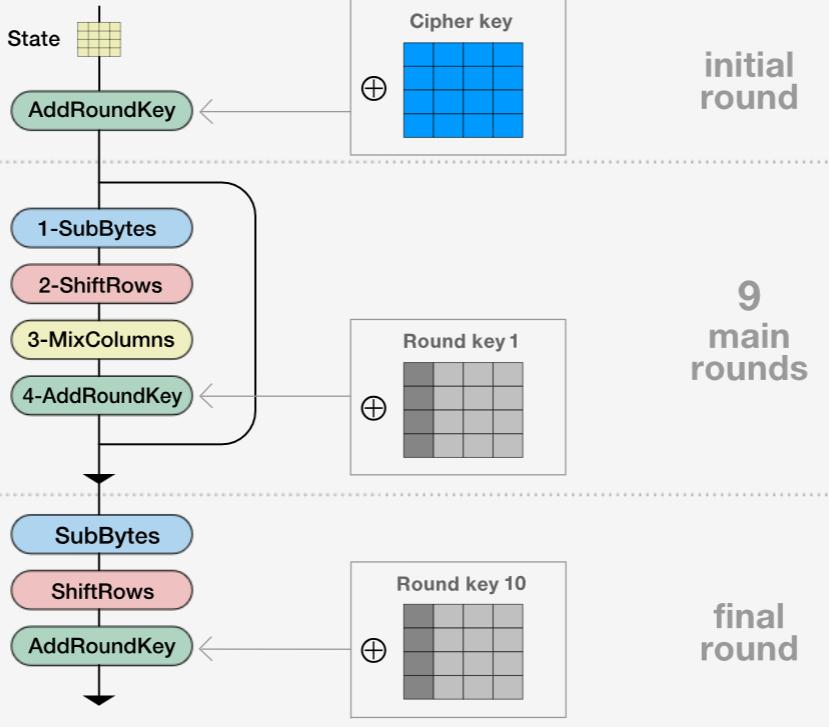
\includegraphics[width=0.5\textwidth]{img/aes-encryption-steps.jpeg}
    \caption{AES encryption steps. Source: Forma Estudio.\cite{aesanimation}.}
    \label{fig:aes-encryption-steps}
\end{figure}

The AES algorithm repeatedly applies four types of transformations as depicted in Figure \ref{fig:aes-encryption-steps}.
The figures in this section are from the Rijandael (AES) Animation made by Forma Estudio\cite{aesanimation}.
This animation explains the algorithm much better than my text, but here is my attempt.
The transformations are:
\begin{enumerate}
    \item \b{SubBytes}.
        Uses an S-BOX, i.e., a lookup table.
        Each cell is substituted (changed) with a value from the S-BOX.
        The value is chosen by taking the first byte from the cell to select the row, and taking the second byte to select the column.
    \item \b{ShiftRows}.
        Each row is rotated to the left with its index.
        The first row stays as-is, the second is rotated 1, the third is rotated 2, and the fourth is rotated 3.
    \item \b{MixColumns}.
        Each column is Galois-multiplied by a specific matrix.
        Galois-multiplication is a special type of multiplication, which gives results in the same set as its inputs.
        So this is yet another step to mix bytes up deterministically.
    \item \b{AddRoundKey}.
        The round key is XOR-ed with the current matrix (explained later).
\end{enumerate}

The \b{AddRoundKey} step mentions a round key.
Round key comes from the Key Scheduling part of the Rijandael algorithm.
The cipher key (input of the algorithm) is expanded into eleven partial keys: one for the initial round, nine for the main rounds, and one for the final round.
We can visualize the cipher key as a matrix yet again, and the round keys will be generated to its right, column by column (see: Figure \ref{fig:aes-key-schedul}).
Starting with the cipher key, up until all the columns are generated, the steps below are performed.
Note that, the steps marked with \b{*} are performed only if the column's position is a multiple of 4.
For the rest of the columns, only XOR applies.
\begin{enumerate}
    \item \b{RotWord*}.
         the column is rotated once, in upside direction.
    \item \b{SubBytes*}
        Same as for enctyption, using the same S-BOX.
    \item \b{XOR}
        The column is XOR-ed with the column 4 positions to the left.
    \item \b{Add*}
        The column is summed with a column from a specific constant matrix (Rcon) 
\end{enumerate}

\begin{figure}[htbp]
    \centering
    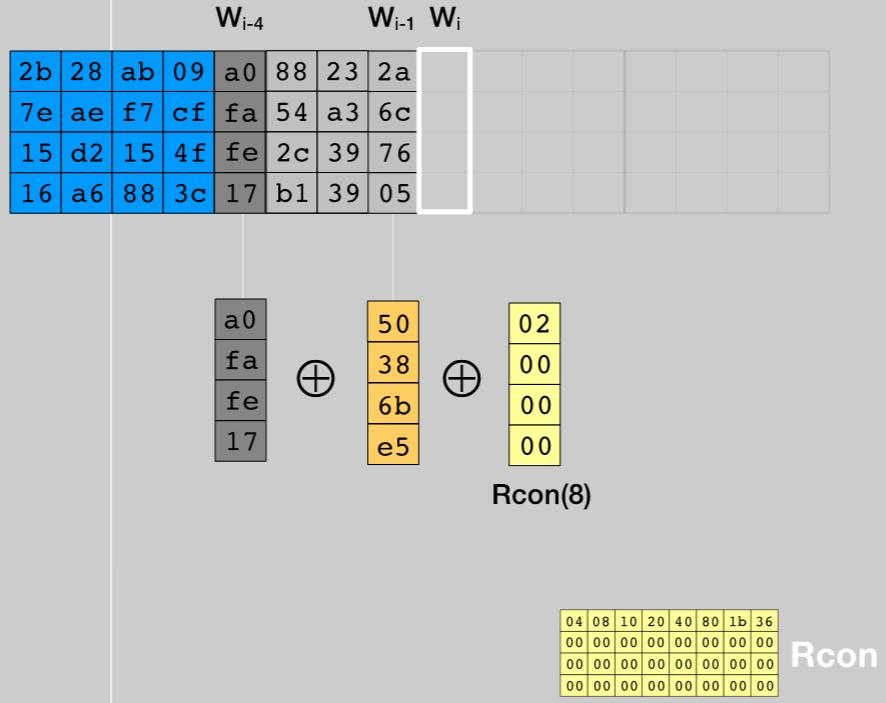
\includegraphics[width=0.5\textwidth]{img/aes-key-schedule.jpeg}
    \caption{AES Key Schedule. Source: Forma Estudio.\cite{aesanimation}.}
    \label{fig:aes-key-schedule}
\end{figure}

Now the amazing part is that encryption can be done the same way, but by reversing everything.
Instead of adding a matrix, we subtract it.
Instead of shifting to one direction, we shift to the opposite direction.
For substitution, we do the inverse substitution.
And Galois-multiplication has its inverse operation as well.
While some of these operations look complicated graphically, computers are really good at performing them, making encryption and decryption fast.
For its strong security, open-source nature and performance, AES is used in almost all cases when symmetric encryption is needed.



\section{Password-Based Key Derivation. PBKDF2} \label{lab:ch3-pbkdf2}



``In cryptography, a key derivation function (KDF) is a cryptographic algorithm that derives one or more secret keys from a secret value such as a master key, a password, or a passphrase using a pseudorandom function (which typically uses a cryptographic hash function or block cipher)''\footnote{\url{https://en.wikipedia.org/wiki/Key_derivation_function}}.
They are often used when keys need to be stretched or need to have a certain format.
A typical use case is applying password-based key derivation on a key before using it for AES.
If the key needs to be of a certain length, depending on the context, just padding it might break the security of the following algorithms, since it is predictable and not random.

Key derivation functions can not only enable random user input to be stretched to the required size, but it usually makes them harder to break as well.
These functions are intentionally slow, so that brute-force attacks and dictionary attacks are harder to be performed if inputs are being guessed.
If the key derivation is deliberately slow enough, it can be considered a hash function.
Such algorithms are, for example, crypt, bcrypt and scrypt.

The Password-Based Key Derivation Functions are examples of key derivation functions.
I used the word in plural since there are to major versions of it, PBKDF1 and PBKDF2.
``PBKDF1 applies a hash function, which shall be MD2, MD5 or SHA-1, to derive keys.
The length of the derived key is bounded by the length of the hash function output, which is 16 octets for MD2
   and MD5 and 20 octets for SHA-1.
(\dots)
PBKDF2 applies a pseudorandom function to derive keys. The length of the derived key is essentially unbounded.''\cite{pbkdf2}

I will focus on PBKDF2, as even the official publication describing them recommends it over PBKDF1.
The PBKDF2 algorithm has the following parameters:
\begin{itemize}
    \item $P$.
        A password, as an octet string (input).
        This is the password from which we want to derive a key.
        Usually user input, and we cannot rely on it being of a specific length or ``strength''.
    \item $S$.
        A salt, as an octet string (input).
        Just as usually, the salt has the purpose to bring randomness to the output.
        Even if the same password is provided, given that the salt is different, the hash will be different.
        This is a mechanism against brute-force and dictionary attacks.
    \item $c$.
        An iteration count, as a positive integer (input).
        It serves the purpose of increasing the cost of producing keys from a password.
        This way it also increases the difficulty of attack, making brute-forcing or building a dictionary take more time.
        The recommended minimum number of iterations is 1000.
    \item $dkLen$.
        The desired length of the derived key (input).
        This depends on what we want the key to use for later.
        But as principle, it can be different numbers, so the algorithm is capable of deriving different length keys.
    \item $PRF$
        The underlying pseudorandom function.
        Depending on which pseudorandom function is used, it might consume different length octets at a time.
        This length is refered to as $hLen$
\end{itemize}

First, the number of $hLen$-octet blocks of the derived key is calculated.
We simply take the total desired length and divide with the length taken at once, and ceil the result.
\begin{equation}
l = \left\lceil \frac{dkLen}{hLen} \right\rceil
\end{equation}

The number of leftover octets (for the last block) will be denoted with $r$.
\begin{equation}
r = dkLen - (l - 1) \times hLen
\end{equation}

Each block of the derived key ($T_i$) will come from the function $F$.
\begin{equation}
T_i = F(P, S, c, i) \quad \text{for } i = 1, 2, \dots, l
\end{equation}

And the function $F$ is the XOR of the first $c$ iterations.
\begin{equation}
F(P, S, c, i) = U_1 \oplus U_2 \oplus \dots \oplus U_c
\end{equation}

Where each iteration $U_i$ comes from applying $PRF$ on the password and different salts.
For the first iteration, the salt is $S$ concatenated with an encoded version of $i$ (the block index).
For the rest of the blocks, the salt is the result of the previous iteration.

\begin{align}
U_1 &= \operatorname{PRF}(P, S \parallel \operatorname{INT}(i)) \nonumber \\
U_2 &= \operatorname{PRF}(P, U_1) \nonumber \\
&\vdots \nonumber \\
U_c &= \operatorname{PRF}(P, U_{c-1})
\end{align}

After each block is calculated, they are concatenated.
From the last block we only take the first $r$ octets.
The result is the derived key, having the desired length.
\begin{equation}
DK = T_1 \parallel T_2 \parallel \dots \parallel T_l \langle 0 \dots r-1 \rangle
\end{equation}


\section{Hashing and Argon2} \label{lab:ch3-argon2}

``Hashing is a process that converts any input to a fixed-length, seemingly random output.''\footnote{\url{https://www.bitdefender.com/en-us/business/infozone/what-is-hashing}}.
For a function to be called hashing function, it has to fulfill certain criteria, aside of giving the same length output for any length input.
First of all, it has to be a one-way function.
Unlike for encryption, where we want the ciphertext to be decryptable, in case of hashing, it shall be impossible to convert the output of a hash function back to the input which it came from.
Hashes are compared between each other, or used as they are, but never reversed.

Then, it has to have good collision resistance.
Since we convert to a fixed size string, multiple inputs will give the same output, inevitably.
It is like parking infinite cars, in seemingly random order, into finite parking lots.
At one point, parking lots will fill up, and two cars will have the same lot.
This means that, if used for password storage and authentication, there is a mathematical chance that two passwords give the same hash, even with salting.
This would mean logging in with an incorrect password.
The catch is that for hash functions with good collision resistance, the chances are terribly low.
For example, for the MD5 algorithm, which was broken in 2004 (it was shown that it is not collision-resistant), the probability to have two passwords producing the same hash is $\frac{1.47}{10^{29}} = 0.0000000000000000000000000000147\%$.\footnote{\url{https://infosecscout.com/two-passwords-same-hash/}}.

The third criterion for a hash function to be considered usable is to be deterministic, not random.
That is why, in the last paragraph's analogy, I said ``seemingly random''.
The same input must give the same output all the time.
Otherwise, it would just be a random number generator, without the current practical use cases.

Hash functions are used for various purposes, out of which the most common are:
\begin{itemize}
    \item \b{Password storage.}
        Databases are often leaked, so storing the hash of a password instead clear text is the 101 of cybersecurity.
        In this case, it is extremely important to use a strong hashing algorithm, with proven collision resistance.
    \item \b{Fast look-up data structures.}
        Hash maps, for example, are often used where data has to be retrieved in \t{O(1)} time complexity.
        If we want to look for something, we compute its hash, which is the address it is supposed to be at.
        This way, we can instantly look up data.
        Collision resistance in this use-case is important for maintaining the speed advantage, not for security.
    \item \b{File signatures.}
        A hash function can take the contents of a whole file and convert it into a much shorter hash.
        This way, we get a unique value, a signature for each file (again, given that no collisions happen).
        We can easily check if a file changed, by looking at the previous and current signature.
        File signatures are also used for static malware analysis: we can take the hash of a program, feed it to a database like \url{https://www.virustotal.com}, and check if it is a reported malware.
\end{itemize}

Argon2\cite{argon2} is a password hashing algorithm, the winner of the Password Hashing Competition.
``PHC ran from 2013 to 2015 as an open competition—the same kind of process as NIST's AES and SHA-3 competitions, and the most effective way to develop a crypto standard.
We received 24 candidates, including many excellent designs, and selected one winner, Argon2, an algorithm designed by Alex Biryukov, Daniel Dinu, and Dmitry Khovratovich from University of Luxembourg.''\footnote{\url{https://www.password-hashing.net/}}.

The algorithm aims to maximize the cost of password cracking on Application-Specific Integrated Circuits (ASICs).
An ASIC is An ``integrated circuit designed for a specific customer, application, or market (\dots) interconnected, and simulated to provide the desired system functions and level of performance.'' \footnote{\url{https://www.analog.com/media/en/analog-dialogue/volume-24/number-3/articles/volume24-number3.pdf\#page=12}}.
In this context, it refers to hardware specialized for password cracking.
The advanced attackers who use such software often exploit parallelization (on GPUs, FPGAs, with more cores), they compute blocks ahead, they juggle with time-memory tradeoff (``the adversary can trade memory for time and do his job on fast hardware with low memory.''\cite{argon2}).

Argon2 takes all these aspects into account, and comes with a solution in two flavors: Argon2d and Argon2i.
Argon2d is faster and uses data-depending memory access, suitable for cryptocurrencies, for example.
Argon2i is slower and uses data-independent memory access, which is preferred for password hashing.
Data-dependent indexing takes into account the password when choosing the memory index to write to, this way making it impossible to prefetch and precompute missing data.
Some software, like Bitwarden, use Argon2id, which uses ``a combination of data-depending and data-independent memory accesses, which gives it some of Argon2i's resistance to side-channel cache timing attacks and much of Argon2d's resistance to GPU cracking attacks.''\footnote{\url{https://bitwarden.com/help/kdf-algorithms/}}

The mathematics behind Argon2 are out of scope for this document, but simply said, the algorithm consists of three steps.
First, memory initialization fills a defined memory size with pseudorandom values derived from the password, salt, and other parameters.
Then, the memory's contents are repeatedly combined with the password and the salt.
After all the iterations, the used memory is compressed into a fixed-size output (the hash).\footnote{\url{https://jumpcloud.com/it-index/what-is-argon2}}.
All this makes Argon2 an outstanding choice for password hashing, proven to be up-to-date with today's attackers.




\section{Full Disk Encryption and LUKS} \label{lab:ch3-luks}

Full disk encryption, as its name suggests, refers to encrypting every byte of a physical disk.
This mechanism is especially powerful since it provides a layer of security for the whole contents of a machine.
It also works for removable media.
With full disk encryption, an attacker's physical access does no longer mean compromised data.
With powerful encryption, brute-forcing decryption of a full disk takes so much time that it is virtually impossible.
``LUKS (Linux Unified Key Setup) is the standard disk encryption format for Linux, built on top of the dm-crypt kernel module.
It is the encryption layer used by default when you select “encrypt disk” during installation on Fedora, Ubuntu, Debian, and most other major distributions.''\footnote{\url{https://secure-os.org/articles/luks-encryption/}}.

It uses PBKDF2 to enhance weak user passwords and has a two level key hierarchy.\cite{luks}
This means that a master password is generated, which is not shared with the user, and the user's password is used to encrypt this master password, which is then stored in a slot.
There are several such slots (key material sections) in the LUKS header, meaning that multiple passwords can be used to decrypt the disk.
As a result, one can have a recovery key along the usual user password.

The LUKS header is the first few bytes of the disk which contains metadata needed for decryption (the algorithm, the KDF etc.).
It is a good idea to have a periodic backup of the LUKS header, since if this part of the memory is damaged, the whole disk becomes inaccessible.
It is a single point of failure, but there is no free meal.

LUKS2, the newer variant of LUKS, is a good option for encrypting disks and USB devices.
As with other cryptographic algorithms, there have been vulnerabilities in their implementation: in 2016, you could gain access by simply holding the enter button.\footnote{\url{https://hmarco.org/bugs/CVE-2016-4484/CVE-2016-4484_cryptsetup_initrd_shell.html}}.
But it is a good standard, and its open-source implementation is patched regularly.



\section{TPM} \label{lab:ch3-tpm}

``A Trusted Platform Module, also known as a TPM, is a cryptographic coprocessor that is present on most commercial PCs and servers'' \cite{tpmbook}.
This chip provides hardware-backed cryptographic primitives upon which software applications can build on.
Usually, when TPM is mentioned, it refers to the chip, which can come from different manufacturers, but must implement the specification defined by the Trusted Computing Group.

There are two main TPM specifications, one of them being TPM 1.2 (ISO/IEC 11889:2009) and the newer one being TPM 2.0 (ISO/IEC 11889:2015).\footnote{\url{https://en.wikipedia.org/wiki/Trusted_Platform_Module}}.
TPM 2.0 is not backward compatible with TPM 1.2.
While both specify similar features, TPM 2.0 is broader and is being pushed over its predecessor.
Since 2016, Microsoft has required all new PCs shipping with Windows 10 to include TPM 2.0 support.
When they released Windows 11 in 2021, the requirements contained TPM 2.0 support.
This caused major backlash, since many older PCs did not (and still do not) have this.
It is hard to find up-to-date exact statistics related to TPM 2.0 adoption rate, probably the least speculative number comes from Windows 11 adoption, as published by Microsoft (given that we trust them).
In March the 3rd, 2026, they stated that ``Windows 11 Dominates Desktop Share in 2026: ~73\% of Windows PCs''.\footnote{\url{https://windowsforum.com/windows-news.4/windows-11-dominates-desktop-share-in-2026-73-of-windows-pcs.403819/?spm=a2700.accio_bizSeo.0.0.180331dah3UXgl}}.
We can assume that most of these machines have TPM 2.0 (with some technical knowledge, or endorsement from Microsoft, this requirement can be bypassed).

A TPM is often refered to as a cryptographic coprocessor, a hardware security module (HSM) or a hardware root of trust (HToT).\cite{tpmpdf}
Its cryptographic functionalities include Random Number Generation (RNG), key generation, provides hashing functions and Hash Based Message Authentication Code (HMAC), as well as implementations for SHA-1, SHA-256, SHA-384, RSA,
ECC, AES, SM4 and XOR.
It also comes with volatile and non-volatile memory.
Volatile memory is used for authorization sessions and storing active keys.
Non-volatile memory has modules such as the Platform Configuration Registers (PCRs) and a limited Non-Volatile Random Access Memory (NVRAM).

The primary scope of TPM is to verify integrity during the boot process.
Its PCRs contain values which can be used ``to cryptographically record (measure) software state: both the software running on a platform and configuration data used by that software.''\cite{tpmbook}.
The state is hashed and the hash is used when booting to verify is the system was altered or not.

The NVRAM is used to store two types of data: data structures defined by the TPM architecture and unstructured data defined by a user.
An example use case mentioned by \cite{tpmbook} is storing a secret.
This memory is very limited in size, so it is not for storing large files.
Instead, the encryption key for a large file could be stored.

All in all, TPM 2.0 provides various hardware-backed cryptographic primitives, which could be used by the OS, but also by software running on a machine.
The TPM in itself is not a solution to all security problems neither.
Probably the biggest criticism of it came from the VeraCrypt developers, stating that ``The only thing that TPM is almost guaranteed to provide is a false sense of security.''\footnote{\url{https://veracrypt.io/en/FAQ.html}}.
Indeed, if the device is stolen, it is just a matter of time, technical skills and available resources before it is bypassed.
However, using its cryptographic primitives instead of software solutions is undoubtably stronger, with one catch - we have to trust the TPM manufacturer and vendor.
